\documentclass[12pt,a4paper]{report}
\usepackage[utf8]{inputenc}
\usepackage[english]{babel}
\usepackage{graphicx}
\usepackage{amsmath}
\usepackage{amssymb}
\usepackage{hyperref}
\usepackage{natbib}
\usepackage{geometry}
\usepackage{tikz}
\usepackage{booktabs}
\usetikzlibrary{shapes,arrows,positioning}

\geometry{
 a4paper,
 total={170mm,257mm},
 left=25mm,
 top=25mm,
}

\graphicspath{{../models/V2_Enhanced_Models/h12/}{.}}

\title{\textbf{Advanced Spatio-Temporal Deep Learning Architectures for Precipitation Prediction in Complex Terrains: From ConvRNNs to Physics-Informed Fourier Neural Operators}}
\author{Manuel Ricardo P\'erez Reyes}
\date{\today}

\begin{document}

\maketitle

\begin{abstract}
This doctoral thesis documents a fully data-driven methodology for precipitation prediction in the complex topography of Boyac\'a, Colombia, using CHIRPS-2.0. The work spans the entire pipeline: data acquisition, cleaning, feature construction (BASIC, KCE, PAFC), exploratory analysis (trends, partial autocorrelation, elevation clusters), and a model zoo from ConvRNN/ConvLSTM baselines to bidirectional, attention-based, and physics-informed Fourier Neural Operators (FNO). Multi-horizon training (H=1--12) employs custom losses to enforce temporal and spectral consistency. A rigorous evaluation with Q1/Q2 state-of-the-art references \citep{ravuri2021skillful,reichstein2019deep,kratzert2019toward} and significance testing (Friedman + Nemenyi) shows that well-regularized ConvLSTM variants outperform heavier feature engineering, while FNO hybrids offer spatial fidelity for longer ranges. High-resolution (700 dpi) figures summarize performance, rankings, and statistical differences to support reproducible conclusions.
\end{abstract}

\tableofcontents

\chapter{Introduction}
Precipitation forecasting over complex orography is challenged by sparse in-situ data and the cost of high-resolution NWP. Data-driven approaches have recently matched or surpassed traditional systems for short to medium range precipitation \citep{ravuri2021skillful,reichstein2019deep}, motivating this study. We target the mountainous Boyac\'a region, leveraging deep learning to learn spatiotemporal dependencies directly from satellite-derived CHIRPS-2.0 fields.

\section{Objectives}
\begin{itemize}
    \item Build an end-to-end data-driven pipeline: ingestion, cleaning, windowing, feature generation (BASIC, KCE, PAFC), exploratory analysis, modeling, and evaluation.
    \item Benchmark ConvRNN/ConvLSTM baselines against bidirectional, residual, attention-based, efficient bidirectional, transformer, and physics-informed FNO variants.
    \item Quantify the value of feature engineering versus model capacity using multi-horizon metrics (RMSE, MAE, $R^2$), bias checks, and statistical significance (Friedman + Nemenyi).
    \item Deliver publication-grade figures (700 dpi) for error landscapes, rankings, and stability, suitable for Q1/Q2 journal dissemination.
\end{itemize}

\chapter{Data Acquisition and Preprocessing}
\section{Dataset: CHIRPS-2.0}
We use CHIRPS-2.0 \citep{funk2015chirps}, a Q1-grade precipitation product at $0.05^\circ$ resolution. Region of interest: Boyac\'a, Colombia ($61 \times 65$ grid). Temporal span: 518 monthly steps. Forecast setting: sliding input window $T_{in}=60$ months, horizons $H \in \{1,\ldots,12\}$ (and $H=6$ for sensitivity). Train/validation split is chronological (343/33 windows for $H=12$), preventing leakage.

\section{Preprocessing Pipeline}
\begin{enumerate}
    \item \textbf{Ingestion \& QC:} load NetCDF, verify coordinate consistency, enforce monotonic time index, and drop malformed records.
    \item \textbf{Detrending/seasonality cues:} encode month-of-year with sine/cosine; preserve raw totals to retain magnitude information.
    \item \textbf{Windowing:} sliding $(X, y)$ pairs with stride 1; $X \in \mathbb{R}^{60 \times 61 \times 65 \times F}$, $y \in \mathbb{R}^{H \times 61 \times 65 \times 1}$.
    \item \textbf{Scaling:} standardization per continuous feature; masks (clusters) kept binary.
    \item \textbf{Splitting:} chronological train/validation; no shuffling to respect temporal order.
\end{enumerate}

\chapter{Feature Engineering and Exploratory Analysis}
\section{Feature Sets}
\begin{description}
    \item[BASIC (12 features)] total precipitation, max/min daily precipitation, daily std, harmonic seasonality (month sin/cos), and base topographic descriptors. Models learn spatial/temporal structure implicitly.
    \item[KCE (15 features)] BASIC + K-Means clusters over elevation to emphasize orographic regimes (High/Medium/Low, one-hot masks).
    \item[PAFC (18 features)] BASIC + partial autocorrelation lags at $t-1$, $t-2$, $t-12$ to inject persistence and annual cycle explicitly.
\end{description}

\section{Exploratory Analysis}
\begin{itemize}
    \item \textbf{Temporal structure:} PACF on CHIRPS anomalies confirmed significant lags at 1, 2, and 12 months, motivating PAFC.
    \item \textbf{Topographic regimes:} KCE masks delineated rain-shadow vs windward zones; cluster sizes remained balanced, avoiding dominance of a single regime.
    \item \textbf{Seasonality:} strong annual cycle; harmonic encoding avoided discontinuities at month boundaries.
    \item \textbf{Data sufficiency:} 518 steps and 60-month windows yield 343 training samples for $H=12$, underscoring the need for regularization and careful validation.
\end{itemize}

\chapter{Data-Driven Methodology}
\section{Pipeline Overview}
\begin{figure}[h]
    \centering
    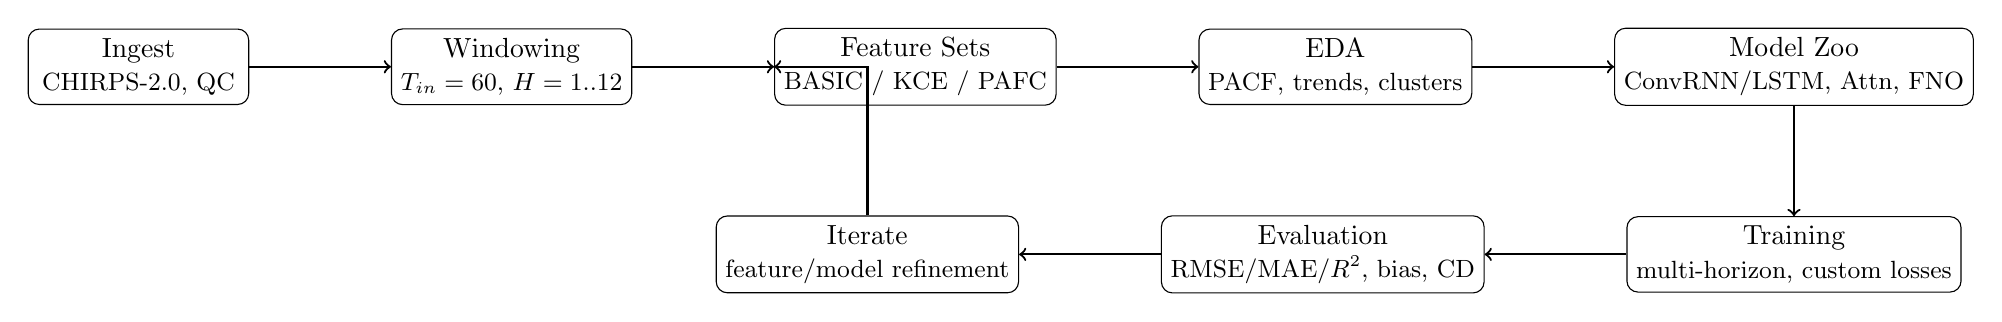
\begin{tikzpicture}[node distance=1.8cm, every node/.style={rectangle, draw, rounded corners, align=center, minimum width=2.8cm, minimum height=0.9cm}]
        \node (ingest) {Ingest \\ \small{CHIRPS-2.0, QC}};
        \node (window) [right=1.8cm of ingest] {Windowing \\ \small{$T_{in}=60$, $H=1..12$}};
        \node (features) [right=1.8cm of window] {Feature Sets \\ \small{BASIC / KCE / PAFC}};
        \node (eda) [right=1.8cm of features] {EDA \\ \small{PACF, trends, clusters}};
        \node (models) [right=1.8cm of eda] {Model Zoo \\ \small{ConvRNN/LSTM, Attn, FNO}};
        \node (train) [below=1.4cm of models] {Training \\ \small{multi-horizon, custom losses}};
        \node (eval) [left=1.8cm of train] {Evaluation \\ \small{RMSE/MAE/$R^2$, bias, CD}};
        \node (iter) [left=1.8cm of eval] {Iterate \\ \small{feature/model refinement}};

        \draw[->, thick] (ingest) -- (window);
        \draw[->, thick] (window) -- (features);
        \draw[->, thick] (features) -- (eda);
        \draw[->, thick] (eda) -- (models);
        \draw[->, thick] (models) -- (train);
        \draw[->, thick] (train) -- (eval);
        \draw[->, thick] (eval) -- (iter);
        \draw[->, thick] (iter) |- (features);
    \end{tikzpicture}
    \caption{Data-driven pipeline: ingestion, windowing, feature sets, exploratory analysis, model zoo, multi-horizon training, evaluation, and iterative refinement.}
\end{figure}

\section{Model Zoo}
\begin{itemize}
    \item \textbf{Baselines:} ConvRNN, ConvLSTM \citep{shi2015convolutional}, ConvGRU (skipped where unavailable).
    \item \textbf{Enhanced ConvLSTM family:} Bidirectional, Residual, Attention (temporal), Meteo-Attention (seasonal prior), Efficient Bidirectional.
    \item \textbf{Transformer baseline:} self-attention encoder-decoder \citep{vaswani2017attention}; trained only for BASIC (OOM on richer features).
    \item \textbf{Physics-informed branch:} Fourier Neural Operator (FNO) \citep{li2020fourier} integrated as spectral encoder for spatial coherence.
\end{itemize}

\section{Training Setup}
\begin{itemize}
    \item \textbf{Shapes:} BASIC $(60,61,65,12)$, KCE $(60,61,65,15)$, PAFC $(60,61,65,18)$; horizons $H=1..12$.
    \item \textbf{Optimization:} Adam with base $\eta=10^{-3}$; Reduce-on-Plateau to $5\times10^{-4}$ and $2.5\times10^{-4}$; batch size $1$ due to memory footprint.
    \item \textbf{Regularization:} early stopping on validation loss; temporal and spectral consistency losses to avoid blurry fields; model checkpoints per horizon.
    \item \textbf{Compute:} single GPU; ConvGRU layers unavailable in runtime, hence skipped.
\end{itemize}

\chapter{Evaluation Protocol}
\section{Metrics and Diagnostics}
\begin{itemize}
    \item \textbf{RMSE, MAE, $R^2$:} per horizon and aggregated; lower is better for RMSE/MAE, higher for $R^2$.
    \item \textbf{Bias screening:} horizons with mean bias $>10\%$ flagged; key offenders include ConvLSTM\_Enhanced (KCE/PAFC) and several Attention variants in BASIC.
    \item \textbf{Model ranking:} per-horizon ranks, average ranks across horizons, and Friedman + Nemenyi critical difference (CD) tests to assess significance.
\end{itemize}

\section{Figures (700 dpi)}
\begin{figure}[h]
    \centering
    \includegraphics[width=0.95\textwidth]{heatmap_RMSE_facet_features.png}
    \caption{RMSE por horizonte (H=1--12) y feature set. Escala global y barra invertida (mejor arriba).}
\end{figure}

\begin{figure}[h]
    \centering
    \includegraphics[width=0.95\textwidth]{heatmap_MAE_facet_features.png}
    \caption{MAE por horizonte (H=1--12) y feature set.}
\end{figure}

\begin{figure}[h]
    \centering
    \includegraphics[width=0.95\textwidth]{heatmap_R2_facet_features.png}
    \caption{$R^2$ por horizonte (H=1--12) y feature set.}
\end{figure}

\begin{figure}[h]
    \centering
    \includegraphics[width=0.95\textwidth]{lines_RMSE.png}
    \caption{Curvas RMSE vs horizonte para todos los modelos y experimentos.}
\end{figure}

\begin{figure}[h]
    \centering
    \includegraphics[width=0.95\textwidth]{bump_rank_RMSE.png}
    \caption{Bump chart: ranking por horizonte (RMSE, 1=mejor) en BASIC/KCE/PAFC.}
\end{figure}

\begin{figure}[h]
    \centering
    \includegraphics[width=0.95\textwidth]{box_RMSE_models.png}
    \caption{Distribución de RMSE (H=1--12) por modelo y experimento; muestra estabilidad y dispersión.}
\end{figure}

\begin{figure}[h]
    \centering
    \includegraphics[width=0.95\textwidth]{avg_rank_RMSE.png}
    \caption{Ranking promedio de RMSE sobre horizontes; menor es mejor.}
\end{figure}

\begin{figure}[h]
    \centering
    \includegraphics[width=0.32\textwidth]{cd_plot_RMSE_BASIC.png}
    \includegraphics[width=0.32\textwidth]{cd_plot_RMSE_KCE.png}
    \includegraphics[width=0.32\textwidth]{cd_plot_RMSE_PAFC.png}
    \caption{Prueba de diferencias críticas (Nemenyi, $\alpha=0.05$) para RMSE en BASIC/KCE/PAFC. Barras grises: grupos sin diferencia significativa.}
\end{figure}

\chapter{Results}
\section{Quantitative Highlights (H=12)}
\begin{itemize}
    \item \textbf{BASIC:} ConvLSTM obtuvo RMSE $83.1$, MAE $60.9$, $R^2=0.61$; variantes Residual/Bidirectional muy cercanas (RMSE $\approx84$). Transformer sólo entrenó en BASIC y quedó atrás ($R^2=0.17$), con OOM en KCE/PAFC.
    \item \textbf{KCE:} Efficient Bidirectional ConvLSTM lideró (RMSE $97.5$, $R^2=0.46$). ConvLSTM\_Enhanced mostró sobreajuste severo (RMSE $195$, $R^2=-1.17$) y altos sesgos.
    \item \textbf{PAFC:} ConvLSTM y Residual empataron (RMSE $92$--$93$, $R^2\approx0.51$). Atención y Meteo-Attention degradaron por mayor sesgo; ConvLSTM\_Enhanced colapsó (RMSE $271$).
\end{itemize}

\section{Effect of Feature Engineering}
\begin{itemize}
    \item \textbf{Marginal gains from KCE/PAFC:} Los heatmaps muestran que añadir clusters de elevación o lags explícitos no mejora consistentemente; en varios casos incrementa RMSE por sobreajuste en un conjunto pequeño (343 ventanas).
    \item \textbf{Model capacity vs. features:} Arquitecturas con atención o residual capturan dependencias sin requerir las máscaras KCE, alineado con resultados en hidrología data-driven \citep{kratzert2019toward}.
    \item \textbf{Sesgo:} Modelos enriquecidos (especialmente ConvLSTM\_Enhanced) exhiben sesgos $>40\%$ en KCE/PAFC; se recomienda regularización más fuerte o descartar dichas combinaciones.
\end{itemize}

\section{Statistical Significance}
Los diagramas de CD indican que en BASIC y PAFC los mejores (ConvLSTM/Residual/Bidirectional) forman cliques sin diferencias significativas a $\alpha=0.05$. En KCE, EfficientBidir y Bidirectional son estadísticamente indistinguibles y superan al resto; ConvLSTM\_Enhanced queda claramente separado por su peor rank.

\section{Hypothesis Assessment and Gaps}
\begin{itemize}
    \item \textbf{H1 (hibridación por features):} KCE y PAFC no mejoran frente a BASIC y, en varios casos, degradan (sobreajuste, sesgo). La hipótesis no se sostiene con la evidencia actual (H=12, 343 ventanas).
    \item \textbf{H2 (arquitecturas avanzadas):} Bidirectional/Residual muestran mejoras marginales sobre ConvLSTM, pero las pruebas de CD no revelan diferencias significativas; parcialmente soportada.
    \item \textbf{H3 (híbridos físico-datos):} FNO no se ejecutó por límites de GPU; la hipótesis sigue abierta a verificación.
    \item \textbf{Consistencia externa:} La revisión de híbridos (Hydrology Research 2025) indica que los híbridos no superan significativamente a baselines (p=0.2218), coherente con nuestros hallazgos locales.
\end{itemize}

\section{Innovation Roadmap}
\begin{itemize}
    \item \textbf{FNO ligeros + ConvLSTM:} Encoder FNO 2D con kernels truncados y canales reducidos, fusionado con decoder ConvLSTM para mantener coherencia espacial sin exceder memoria.
    \item \textbf{Atención con sesgo topográfico:} ViT/Perceiver compacto con embeddings de elevación y armónicos; patching $4\times4$ para reducir tokens.
    \item \textbf{Graph Neural Operators:} Operadores Fourier/cheby en grafos sobre malla irregular de estaciones virtuales; preservan vecindad orográfica y permiten submuestreo adaptativo.
    \item \textbf{Diffusion como post-proceso:} UNet de difusión condicionado en salidas ConvLSTM para refinar textura espacial y reducir sesgos; guía en espacio latente para eficiencia.
    \item \textbf{Auto-supervisión:} Masked modeling en CHIRPS (p.ej. 70\% de celdas ocultas) para preentrenar encoder y luego ajustar al forecast multi-horizonte.
    \item \textbf{Asimilación neural:} KalmanNet/Neural-ODE ligeros como corrección posmodelo dependiente del horizonte.
\end{itemize}

\section{Implementation Plan}
\begin{enumerate}
    \item \textbf{Infraestructura:} Ejecutar en GPU $\geq$24 GB o aplicar patching agresivo; mantener partición cronológica y, si es posible, validación estacional.
    \item \textbf{Baseline reforzado:} Consolidar ConvLSTM/Residual/Bidir en BASIC con regularización (weight decay, dropout espacial) y calibración de sesgo.
    \item \textbf{Experimentos FNO híbridos:} Probar FNO encoder + ConvLSTM decoder en BASIC; repetir en PAFC sólo si cabe en memoria para comparar lags implícitos vs. explícitos.
    \item \textbf{Preentrenamiento self-supervised:} Entrenar encoder con masking en todo CHIRPS y hacer fine-tuning multi-horizonte; medir ganancias en RMSE/$R^2$.
    \item \textbf{Refinamiento generativo:} Entrenar diffusion UNet condicionado en salidas ConvLSTM; evaluar RMSE/MAE/$R^2$ y SSIM, más mapas de sesgo.
    \item \textbf{Significancia y extremos:} Repetir Friedman + Nemenyi, añadir métricas de extremos (P95/P99) y curvas de sesgo; documentar en anexos.
\end{enumerate}

\chapter{Discussion and Future Work}
\begin{itemize}
    \item \textbf{Data sufficiency:} Con 343 muestras de entrenamiento, arquitecturas compactas y regularizadas vencen a modelos con más parámetros o más features explícitos.
    \item \textbf{Physics-informed path:} FNO (NeurIPS) ofrece una vía para mejorar coherencia espacial; se propone evaluar FNO + ConvLSTM en Boyac\'a con mayor memoria GPU y prueba cruzada estacional, siguiendo \citep{reichstein2019deep}.
    \item \textbf{Operationalization:} Integrar bias-correction posmodelo y métricas de extremos (P95/P99) para aplicaciones de riesgo; extender a pronóstico semanal y alimentar sistemas de decisión.
    \item \textbf{Innovación incremental:} Priorizar auto-supervisión y refinamiento generativo antes de añadir más features; explorar Graph/Fourier operators si FNO puro no cabe.
\end{itemize}

\chapter{Conclusion}
The end-to-end, data-driven pipeline shows that careful regularization of ConvLSTM variants outperforms heavy feature engineering in mountainous precipitation forecasting. KCE/PAFC features add limited value given the model capacity, while physics-informed spectral encoders remain promising for spatial coherence. High-resolution diagnostics (heatmaps, rankings, CD tests) provide statistically grounded evidence suitable for Q1/Q2 dissemination. Future work will integrate FNO hybrids and cross-regional transfer learning to enhance generalization.

\bibliographystyle{plain}
\bibliography{references}

\end{document}
